% !TEX TS-program = lualatex
% !TEX encoding = UTF-8 Unicode
% !TEX spellcheck = en_US
% © 2024 Moritz Brinkmann, CC-by-sa
% https://ma.latexkurs.de

\documentclass[
	vorläufig=false,
	datum=2024-03-08,
	titel={day one},
	web=true, handout,
	kursB,
	englisch=true,
]{../tex/latexkurs-slides}

\usepackage{caption,booktabs,siunitx,adjustbox}

\setotherlanguages{german,russian,dutch}


%% Notes:
%% Zitate: Harvard-Methode (AuthorYear)


\begin{document}

\begin{frame}{Learning Objectives}
After the two workshop days, you will be able to:
	\begin{itemize}
		\item create simple documents in \LaTeX
		\item find assistance in class and package documentation
		\item create multilingual documents
		\item incorporate images and create tables
		\item generate reference lists
		\item typeset mathematical formulas
		\item structure larger projects
	\end{itemize}
\end{frame}

\begin{frame}<handout:0>[t]{Logistics}%{General Information}
	\begin{block}<1->{Dates}
		\begin{itemize}
			\item Two sessions:
				\begin{itemize}
				\kursAB{
					\item Saturday, February 15 (today)
					\item Sunday, February 16 (tomorrow)
				}{
					\item Saturday, March 8 (today)
					\item Sunday, March 9 (tomorrow)
				}
				\end{itemize}
			\item Each session from 10 am to 3 pm
			\item Approximately 45 minutes break
		\end{itemize}
	\end{block}
	\begin{block}<2>{Materials}
		\begin{columns}
			\column{.7\textwidth}
				\begin{itemize}
					\item All materials are available on the \href{https://ma.latexkurs.de}{workshop website} or in \href{https://ilias.uni-mannheim.de/goto.php?target=fold_1589856&client_id=ILIAS}{ILIAS} for download:\\[1ex]
					\url{https://ma.latexkurs.de/}\\\quad
				\end{itemize}
			\column{.25\textwidth}
				\vspace*{-2mm}
				
				\begin{minipage}{1.05in}
					\centering
					\textcolor{white}{\rule{0.9in}{0.9in}}\vspace*{-0.86in}
					\qrcode{https://ma.latexkurs.de}
				\end{minipage}
			\end{columns}
	\end{block}
\end{frame}

\begin{frame}<all:0| handout:99>[t]{Logistics}%{General Information}
	\begin{block}{Dates}
		\begin{itemize}
			\item Two sessions per date:
			\vspace*{-1.2ex}
				\begin{columns}
					\column{0.28\textwidth}
					\begin{itemize}\setlength{\itemsep}{0pt}
							\item Saturday, February 15
							\item Sunday, February 16
					\end{itemize}
					\column{0.04\textwidth}
						\emph{or}
					\column{0.26\textwidth}
					\begin{itemize}\setlength{\itemsep}{0pt}
						\item Saturday, March 8
						\item Sunday, March 9
					\end{itemize}
					\column{0.1\textwidth}
						\vspace{1.5cm}
				\end{columns}
%				\vspace{1ex}
			\item Each session from 10 am to 3 pm
			\item Approximately 45 minutes break
		\end{itemize}
	\end{block}
	\begin{block}{Materials}
		\begin{columns}
			\column{.7\textwidth}
				\begin{itemize}
					\item All materials are available on the \href{https://ma.latexkurs.de}{workshop website} or in \href{https://ilias.uni-mannheim.de/goto.php?target=fold_1589856&client_id=ILIAS}{ILIAS}
					 for download:\\[1ex]
					\url{https://ma.latexkurs.de/}\\[1em]\quad
				\end{itemize}
			\column{.25\textwidth}
				\vspace*{-2mm}
				
				\begin{minipage}{1.05in}
					\centering
					\textcolor{white}{\rule{0.9in}{0.9in}}\vspace*{-0.86in}
					\qrcode{https://ma.latexkurs.de}
				\end{minipage}
			\end{columns}
	\end{block}
\end{frame}


\begin{frame}[t]{Organizational Matters}
	\begin{block}{Exercises}
		\begin{itemize}
			\item Theory and practical phases alternate.
			\item You are allowed (and encouraged) to try examples \emph{at any time} on your computer.
			\item Feel free to experiment with something new \emph{immediately}!
			\item Don't hesitate to ask if you're having trouble with anything.
			\item If you are using \href{https://www.overleaf.com?r=60500875&rm=d&rs=b}{Overleaf}, you can share your source code with \href{mailto:overleaf@latexkurs.de}{\texttt{overleaf@latexkurs.de}} when you have questions.
		\end{itemize}
	\end{block}
%	\begin{olcol}
		\begin{block}{\LaTeX\ Flavor}
			The content of this course is based on the (relatively modern) variant \hologo{LuaLaTeX}.
		\end{block}
%	\end{olcol}
%	\overleaf{tex00}
\end{frame}

\begin{frame}[t,allowframebreaks]{Content}
	\tableofcontents
\end{frame}


%%%%%%%%%%%%%%%%%%%%%%%%%%%%%%%%%%%%%%%%%%%%%%%%%%%%%%%%%%%%%%%%%%%%%%%%%%%%%%%%%%%%%%%%%%%%%%%%%%%%%%%%%%
\teil[What is it all about?]{The Name of the Game}
%%%%%%%%%%%%%%%%%%%%%%%%%%%%%%%%%%%%%%%%%%%%%%%%%%%%%%%%%%%%%%%%%%%%%%%%%%%%%%%%%%%%%%%%%%%%%%%%%%%%%%%%%%
\subsection*{\TeX}

\begin{frame}[<+->][t]{The Name of the Game}
	\begin{itemize}
		\item Program \alert{\TeX} (Since 1977)
			\only<1>{\\ Written by Donald E. Knuth for his book "The Art of Computer Programming".
			\\ "TeX" from Greek τέχνη} % téchne, ancient Greek: skill, craftsmanship, art
		\item Macro package \alert{plain}\TeX
			\only<2>{\\ Makes \TeX\ usable for regular users.}
		\item Extended macro package \alert{La}\TeX\ (Early 1980s)
			\only<3>{\\ By Leslie Lamport: "Lamport's \TeX".\\ Many simplifications for the average user.}
		\item Current stable version: \alert{La}\TeX\,\alert{2$_\varepsilon$} (1994)
			\only<4>{\\ "in an $\varepsilon$-environment of 2"}
		\item Future development: \LaTeX{}3 \\ not yet independently available, but as a package \texttt{expl3} in \LaTeXe%\\ (provides \LaTeX{}3 syntax for package authors)
	\end{itemize}		
\end{frame}

\begin{frame}[t]{What is \TeX\ – and what is it not?}
	\only<1>{
		\begin{block}{\LaTeX{} is well-suited for...}
			\begin{itemize}
				%\item Program to write "The Art of Computer Programming"
				\item All documents with a logical structure
				\begin{itemize}
					\item Scientific papers (excellent mathematical typesetting)
					\item Humanities papers (excellent multilingual support, bibliography creation, apparatus creation, etc.)
					\item Articles, bachelor's theses, dissertations, etc.
					\item Book series, letters
					\item Presentations
				\end{itemize}
				\item Much "abuse" by creative package authors
			\end{itemize}
		\end{block}
	}\only<2>{
		\begin{block}{\LaTeX{} is less suitable for...}
			\begin{itemize}
				\item Documents without a logical structure
				\begin{itemize}
					\item Presentations (colorful, rotating, blinking, "chaotic")
					\item Flyers
					\item Posters
				\end{itemize}
				\item Documents with many inconsistent images that are freely moved
			\end{itemize}
		\end{block}
	}
\end{frame}

\begin{frame}{How does \TeX\ work?}
	\begin{itemize}
		\item WYSIWYM
		\item Plain text files
		\item No hidden settings
		\item Text formatting using special commands:
		\begin{itemize}
			\item "I want to write an article!"
			\item "Create a heading!"
			\item "Make the following bold!"
			\item "Create a table that..."
		\end{itemize}
	\end{itemize}
\end{frame}

\begin{frame}[t]{How does \TeX\ work?}
	\begin{columns}[t]
		\begin{column}{.45\textwidth}
			\begin{block}{Advantages}
				\begin{itemize}
					\item Stability and portability
					\item Small file sizes
					\item Editable with any text editor
					\item Text files are always readable
					\item Consistent output everywhere
				\end{itemize}
			\end{block}
		\end{column}
		\begin{column}{.45\textwidth}
			\begin{block}{Disadvantages}
				\begin{itemize}
					\item Result not immediately visible
					\item Non-intuitive interface
					\item Steep learning curve
					\item Changes require recompilation
					\item Complex layout desires are hard to achieve
				\end{itemize}
			\end{block}
		\end{column}
	\end{columns}
\end{frame}

\begin{frame}[fragile]{A simple \TeX\ document}
	How can text be distinguished from commands?\\[1em]
	
	Approach in \emph{classical} programming languages:
\begin{lstlisting}
print ( "Hello, World!" );
\end{lstlisting}
	⇒ unsuitable for a typesetting program
\end{frame}

\begin{frame}[fragile]{A simple \TeX\ document}
	\begin{itemize}
		\item \TeX{} is a markup language
		\item Individual characters have special meanings
		\item Backslash (\verb|\|) serves as an escape character and marks the beginning of a command: \verb|\chapter \section \author|
	\end{itemize}\quad\\[1em]
	Simplest \TeX\ document:
\begin{lstlisting}
Hello, World! \bye 
\end{lstlisting}\quad\\[1em]
	\pause
	\promt|tex document.tex|\\ creates a |.dvi| document and a |.log| file
	% Live demonstration
\end{frame}

\begin{frame}[fragile]{A simple \LaTeX\ document}
\begin{LTXexample}
\documentclass{minimal}
\begin{document}
Hello, World!
\end{document}
\end{LTXexample}
\pause\vfill
\begin{arbeitsauftrag}
Create your first \LaTeX\ document by typing this minimal example in your editor!
\end{arbeitsauftrag}
\end{frame}

\begin{frame}[fragile]{Command Characters}
	\begin{tabular}{ll}
			\verb|\| & \emph{escape character}, marks the beginning of commands \\
			\verb|{}| & \emph{grouping character}, groups related characters together \\& e.g., arguments \verb|\textbf{bold}|\\
			\verb|$| & \emph{math character}, starts and ends math mode \\
			\verb|&| & \emph{tabbing character}, separates columns in tables \\
			\verb|%| & \emph{comment character}, comments out the rest of the line \\
			\verb|^_~#| & other characters with special meaning
	\end{tabular}
\end{frame}


%%%%%%%%%%%%%%%%%%%%%%%%%%%%%%%%%%%%%%%%%%%%%%%%%%%%%%%%%%%%%%%%%%%%%%%%%%%%%%%%%%%%%%%%%%%%%%%%%%%%%%%%%%
\teil{Basic Operation}
%%%%%%%%%%%%%%%%%%%%%%%%%%%%%%%%%%%%%%%%%%%%%%%%%%%%%%%%%%%%%%%%%%%%%%%%%%%%%%%%%%%%%%%%%%%%%%%%%%%%%%%%%%
\subsection{Classes and Packages}
\subsubsection*{Document Classes}

\begin{frame}{Document Classes}
	Document classes define fundamental properties of the document:
	\begin{itemize}
		\item Layout
		\item Default fonts
		\item Page layout
		\item Sectioning commands
		\item Appearance of lists, tables, enumerations, etc.
	\end{itemize}
	Properties can be customized by changing options or loading packages.
\end{frame}

\begin{frame}{Document Classes}
	\begin{tabular}{rl}
		&\kern-1.5cm \bf Standard Classes\\
		article & (Short) articles\\
		report & Reports, conference reports\\
		book & Books\\
		letter & Letters\\
		minimal & For minimal examples\\ \\
		&\kern-1.5cm \bf KOMA-Script\\
		scrartcl & Extension of article\\
		scrreprt & Extension of report\\
		scrbook & Extension of book\\
		scrlttr2 & Very powerful letter class\\ \\
		&\kern-1.5cm \bf Special Classes\\
		beamer & For presentations\\
		tikzposter & Scientific posters
	\end{tabular}
\end{frame}

\subsubsection*{Packages}
\begin{frame}[fragile]{Packages}
\begin{itemize}
\item Packages provide additional functionality
\item Work facilitators
\item Error corrections
\item Include in the preamble using
%\pdfmarginpar[Help]{The preamble is everything between documentclass{} and begin{document}}
|\usepackage[|\meta{option(s)}|]{|\meta{package name}|}|:
\begin{lstlisting}
\documentclass{article}
\usepackage{
  amsmath,
  hyperref,
}
\usepackage[left=2cm]{geometry}
\end{lstlisting}
\end{itemize}
\end{frame}

\begin{frame}[fragile]{Sectioning Commands}
	\begin{itemize}
		\item Sectioning structures organize documents
		\item Enable automatic numbering, entry in tables of contents, column titles, etc.
		\item Defined by the document class
		\item Basic structure defined in the kernel
		\item[⇒] certain elements always available
	\end{itemize}
	\vfill
	\begin{olcol}
\begin{lstlisting}
\teil{Part I}
\chapter{Chapter}
\section{Section}
\subsection{Subsection}
\subsubsection{Subsubsection}
\paragraph{Paragraph}
\subparagraph{Subparagraph}
\end{lstlisting}
	\end{olcol}
	\overleaf*{tex01}
\end{frame}

%\begin{frame}{Selection of Packages}
%	\begin{tabular}{rl}
%		graphics/x & provides (extended) graphics support\\
%		amsmath & Improvements, extensions for math typesetting\\
%		babel/polyglossia & Language support (hyphenation rules, etc.)\\
%		inputenc & Enables various input encodings\\
%		fontenc & Enables various font encodings\\
%		lmodern & Switches to lmodern fonts\\
%		fontspec & Enables the use of system fonts\\
%		tikz & Very powerful drawing environment\\
%		\vdots & \vdots
%	\end{tabular}
%\end{frame}


\begin{frame}[c,fragile]{Basic Commands}{General}
\begin{tabular}{ll}
|\textrm{Serif}| & \textrm{Serif \quad Abcdxyz}\\
|\textit{italic}| & \textrm{\textit{italic \quad Abcdxyz}} \\%(\emph{do not} use |{\it italic}|)\\
|\textsl{slanted}| & \textrm{\textsl{slanted \quad Abcdxyz}}\\
|\textsf{sans-serif}| & \textsf{sans-serif \quad Abcdxyz}\\
|\textbf{bold}| & \textbf{bold \quad Abcdxyz}\\
|\texttt{typewriter}| & \texttt{typewriter \quad Abcdxyz}\\
|\textsc{Small Caps}| & \textsc{Small Caps \quad Abcdxyz}\\
|\emph{emphasis}| & \emph{emphasis \quad Abcdxyz}\\
|\\| & Line break\\
|\par| or blank line & Paragraph break\\
|$E = \frac{p^2}{2m}$| & Inline math mode: $E = \frac{p^2}{2m}$\\
|\[E = \frac{p^2}{2m}\]| & Display math mode: $\displaystyle E = \frac{p^2}{2m}$\\ % Arno: „well that’s cheated …“ ;-)
|\tableofcontents| & Produces table of contents\\
|\today| & Current date
\end{tabular}
\overleaf{tex01}
\end{frame}

\subsection{Basic Commands}

\begin{frame}[c,fragile]{Basic Commands}{Font Sizes}
\begin{tabular}{ll}
|\tiny| & \tiny tiny \\
|\small| & \small small \\
|\normalsize| & \normalsize normal\\
|\large| & \large large\\
|\Large| & \Large larger\\
|\LARGE| & \LARGE even larger\\
|\huge| & \huge huge\\
|\Huge| & \Huge even huge\\
\end{tabular}
%Manual adjustment: |\fontsize{10}{12}\selectfont|
\overleaf{tex01}
\end{frame}

\begin{frame}[c]{Auxiliary Files}
	\begin{tabular}{ll}
		& \bf Input\\
		.tex & \TeX\ file with document text\\ \\
		& \bf Output\\
		.pdf & pdf\TeX\ output or conversion from (x)dvi\\ \\\pause
		& \bf Auxiliary files (write only)\\
		.log & Log file with information, warnings, errors\\ \\\pause
		& \bf Auxiliary files (read and write)\\
		.aux & Auxiliary file with temporary information\\
		.toc & table of contents\\
		.lof & list of figures\\
		.synctex.gz & required for the Sync\TeX\ feature\\
		\vdots & \vdots
	\end{tabular}
\end{frame}


%\subsection{Engines and Formats}
%\begin{frame}{\TeX\ Engines and Formats}{Terminology}
%	\begin{description}
%		\item[engine] The program that performs the actual typesetting work:\\\TeX, \hologo{pdfTeX}, \luaTeX
%		\item[format] A large collection of macros designed to facilitate work:\\plain\TeX, \LaTeX, \hologo{ConTeXt}
%		\item[distribution] A bundle of engines, formats, extensions (packages, modules), and utility programs:\\\TeXlive, Mac\TeX, \MikTeX
%	\end{description}
%\end{frame}
%
%\begin{frame}{\TeX\ Engines and Formats}{Key Engines}
%	\begin{description}
%		\item[\TeX] The original program written by Donald E. Knuth.
%		\item[\hologo{pdfTeX}] Engine that can directly generate PDF files\\Enables many PDF-specific features such as microtypography.
%		\item[\XeTeX] Processes utf8 encoding by default, allows the use of system fonts, and easy text direction changes.
%		\item[\luaTeX] Offers almost everything \XeTeX\ can do and includes the Lua scripting language that can be invoked from the \TeX\ document.
%	\end{description}
%\end{frame}
%
%\begin{frame}[fragile]{\TeX\ Engines and Formats}{Program Names}
%	The executed program determines the engine and format:\\[1em]
%	\begin{description}
%		\item[|pdftex|] \hologo{pdfTeX} engine, plain format
%		\item[|pdflatex|] \hologo{pdfTeX} engine, \LaTeXe\ format
%		\item[|latex|] \hologo{pdfTeX} engine, \LaTeXe\ format, DVI output
%		\item[|xelatex|] \XeTeX\ engine, \LaTeXe\ format
%		\item[|lualatex|] \luaTeX\ engine, \LaTeXe\ format, PDF output
%	\end{description}
%\end{frame}


%%%%%%%%%%%%%%%%%%%%%%%%%%%%%%%%%%%%%%%%%%%%%%%%%%%%%%%%%%%%%%%%%%%%%%%%%%%%%%%%%%%%%%%%%%%%%%%%%%%%%%%%%%
\teil{Basics of Typography}
%%%%%%%%%%%%%%%%%%%%%%%%%%%%%%%%%%%%%%%%%%%%%%%%%%%%%%%%%%%%%%%%%%%%%%%%%%%%%%%%%%%%%%%%%%%%%%%%%%%%%%%%%%
\subsection{Macrotypography}

\begin{frame}{Macrotypography}
	\begin{itemize}
		\item Text Area
		\item Header and Footer
		\item Font Selection
		\item Formatting Spacing
		\item Appearance of Index, Footnotes, etc.
	\end{itemize}
	
	\pause
	\begin{olcol}
		\begin{arbeitsauftrag}
			Download the file \href{https://latexkurs.github.io/MA-en/exercise_layout.tex}{\texttt{exercise\_layout.tex}} from the workshop website. Apply all typographic settings discussed to this file step by step.

			Ideally, choose values that meet the requirements for your upcoming thesis.
		\end{arbeitsauftrag}
	\end{olcol}
	\overleaf{tex02}
\end{frame}

\begin{frame}{Guidelines for Bachelor Theses in Economics}
\begingroup
\renewcommand{\familydefault}{\rmdefault}
\begin{fancyquote}
\vspace{-1ex}
\normalfont\textbf{\Large Style}
\begin{description}[Left and right margin]
\item[Format] one-sided DIN A4
\item[Font Size] \SI{12}{pt}
\item[Line Spread] \SI{1.5}{pt}
\item[Alignment] justified (“Blocksatz”)
\item[Left and right margin] \SI{3}{\centi\meter}
\end{description}
\quoted{\itshape \href{https://www.vwl.uni-mannheim.de/media/Fakultaeten/vwl/Dokumente/20141105_Guidelines.pdf}{Guidelines for Bachelor theses}}
\end{fancyquote}
\endgroup
\end{frame}

\begin{frame}{Text Area}
	The text area refers to the portion of the page covered by the text (as opposed to the margins).
	\begin{itemize}
		\item Single or double-sided layout?
		\item Font size, line width,
		\item Header and footer
		\item Text columns
	\end{itemize}
\end{frame}


\begin{frame}{Modern Text Area Construction}
	\centering \small
	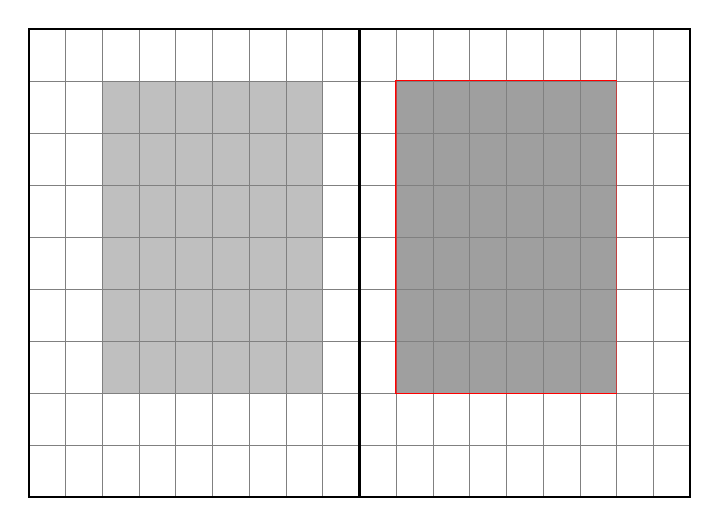
\begin{tikzpicture}
		\coordinate (a) at (-4.20, 5.95);
		\coordinate (b) at ( 0.00, 5.95);
		\coordinate (c) at ( 4.20, 5.95);
		\coordinate (d) at (-4.20, 0.00);
		\coordinate (e) at ( 0.00, 0.00);
		\coordinate (f) at ( 4.20, 0.00);
		
		\coordinate (A2) at ( 0.464, 5.29);
		\coordinate (D2) at ( 3.266, 1.32);
		\coordinate (A2’) at (-0.464, 5.29);
		\coordinate (D2’) at (-3.266, 1.32);

		\draw<1-2>[help lines, xstep=8.4/18, ystep=11.9/18] (a) grid (f);
		
		\draw<2>[red, fill=gray, fill opacity=.5] (A2) rectangle (D2);
		\fill<3>[gray, fill opacity=.5] (A2) rectangle (D2);
		\fill<3>[gray, fill opacity=.5] (A2’) rectangle (D2’);

		\draw [thick]
			(a) rectangle (e)
			(b) rectangle (f);
	\end{tikzpicture}
\end{frame}
%% Markus Kohm: „Satzspiegelkonstruktionen im Vergleich“ http://www.dante.de/tex/Dokumente/KohmSatzspiegel.pdf

\begin{frame}{Text Area in Gutenberg's Printing}
	\hspace{7.00cm}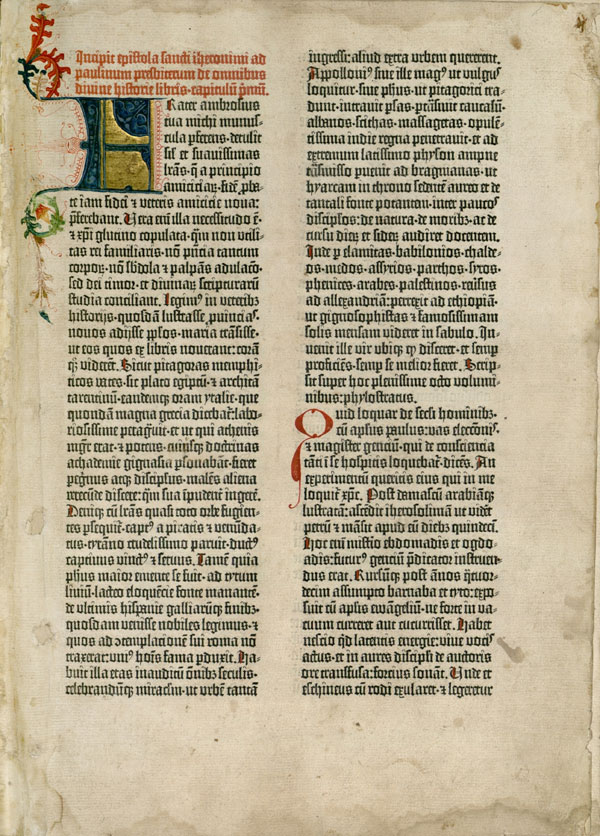
\includegraphics[height=5.95cm]{gutenbergbibel}
\end{frame}

\begin{frame}[fragile]{Text Area with KOMA-Script}
\begin{itemize}
	\item KOMA-Script provides optimal text area construction through its own package \pkg{typearea}.
	\item Adjustment is usually necessary only for exceptionally wide or narrow fonts:
	\\Option |DIV=|\meta{Factor}
	\\Automatic calculation based on page size: |DIV=calc| 
	\\Calculation based on medieval book page canon: |DIV=classic|
	\item Binding correction using option |BCOR=|\meta{Length}
\end{itemize}
\begin{lstlisting}
\documentclass[DIV=9, BCOR=12mm]{scrbook}
\end{lstlisting}
\vfill
\begin{olcol}
For non-KOMA classes, |typearea| must be loaded directly:
\begin{lstlisting}
\usepackage[DIV=13, BCOR=2cm]{typearea}
\end{lstlisting}
\end{olcol}
\end{frame}

\begin{frame}[fragile]{Text Area with |geometry|}
Package \pkg{geometry} allows manual adjustment of the text area:
\begin{lstlisting}
\usepackage[top=2cm, bottom=5cm]{geometry}
\end{lstlisting}
or:
\begin{lstlisting}
\usepackage{geometry}
\geometry{top=2cm, bottom=5cm}
\end{lstlisting}
\end{frame}


\begin{frame}[fragile,t]{Text Area with |geometry|}
\begin{block}{Possible Options}
	\vspace{-1em}
\begin{verbatim}
paper
left, right, inner, outer, hmargin
top, bottom, vmargin
margin
bindingoffset, textwidth, textheight
twocolumn, columnsep, marginparsep, footnotesep
headsep, footsep, nofoot, nohead
hoffset, voffset, offset
includehead, includefoot
\end{verbatim}
\end{block}
%\pause
%\begin{arbeitsauftrag}
%Set the left and right margins of your document to \SI{3}{\centi\meter}.
%\end{arbeitsauftrag}
\end{frame}

\begin{frame}[fragile]{Line Spacing}
Package \pkg{setspace} allows adjustment of line spacing:
\begin{lstlisting}
\usepackage{setspace}
\singlespacing
\onehalfspacing
\doublespacing
\end{lstlisting}
Spacing in footnotes, etc., remains the same.\\
Fine-tuning: |\setstretch{|\meta{Factor}|}|
%\pause
%\begin{arbeitsauftrag}
%Increase the line spacing of your document to \num{1\.5}.
%\end{arbeitsauftrag}
\end{frame}


\subsubsection*{Headers and Footers}
\begin{frame}[fragile, t]{Headers and Footers}
\begin{itemize}
\item Headers and footers contain important information about the document
\begin{itemize}
\item Live column titles
\item Page numbers
\end{itemize}
\item Adjustment using various packages
\item Selection via |\pagestyle{|\meta{page style}|}| or |\thispagestyle{|\meta{page style}|}|
\item Default settings: |empty|, |plain|, |headings|
\end{itemize}
\overleaf{tex03}
\end{frame}

\begin{frame}[fragile, t]{Headers and Footers with scrlayer-scrpage}%
\kern-.7ex The package defines two page styles: |scrheadings| and |screadings.plain|

Adjustment is done through, e.\,g.\\ |\lehead[|\meta{content plain.scrheadings}|]{|\meta{content scrheadings}|}|

\begin{center}\vspace{-1em}\small
\begin{tikzpicture}
		\coordinate (a) at (-.5\textwidth, 3.50);
		\coordinate (b) at ( 0.00, 3.50);
		\coordinate (c) at ( .5\textwidth, 3.50);
		\coordinate (d) at (-.5\textwidth, 2.70);
		\coordinate (e) at ( 0.00, 2.70);
		\coordinate (f) at ( .5\textwidth, 2.70);
		\coordinate (g) at (-.5\textwidth, 0.80);
		\coordinate (h) at ( 0.00, 0.80);
		\coordinate (i) at ( .5\textwidth, 0.80);
		\coordinate (j) at (-.5\textwidth, 0.00);
		\coordinate (k) at ( 0.00, 0.00);
		\coordinate (l) at ( .5\textwidth, 0.00);

		\node (A) at (-3/8*\textwidth, 3.00) {\color{red}|\lehead|};
		\node (B) at (-2/8*\textwidth, 3.00) {\color{green}|\cehead|};
		\node (C) at (-1/8*\textwidth, 3.00) {\color{blue}|\rehead|};
		\node (D) at ( 1/8*\textwidth, 3.00) {\color{blue}|\lohead|};
		\node (E) at ( 2/8*\textwidth, 3.00) {\color{green}|\cohead|};
		\node (F) at ( 3/8*\textwidth, 3.00) {\color{red}|\rohead|};
		
		\node (G) at (-3/8*\textwidth, 0.50) {\color{red}|\lefoot|};
		\node (H) at (-2/8*\textwidth, 0.50) {\color{green}|\cefoot|};
		\node (I) at (-1/8*\textwidth, 0.50) {\color{blue}|\refoot|};
		\node (J) at ( 1/8*\textwidth, 0.50) {\color{blue}|\lofoot|};
		\node (K) at ( 2/8*\textwidth, 0.50) {\color{green}|\cofoot|};
		\node (L) at ( 3/8*\textwidth, 0.50) {\color{red}|\rofoot|};

\only<2>{
		\node (M) at ( 0, 2.6) {\color{blue}\texttt{\textbackslash ihead}};
		\node (N) at ( 0, 2.3) {\color{green}\texttt{\textbackslash mhead}};
		\node (O) at ( 0, 2.0) {\color{red}\texttt{\textbackslash ohead}};
		
		\node (P) at ( 0, 0.9) {\color{blue}\texttt{\textbackslash ifoot}};
		\node (Q) at ( 0, 1.2) {\color{green}\texttt{\textbackslash mfoot}};
		\node (R) at ( 0, 1.5) {\color{red}\texttt{\textbackslash ofoot}};
		
		\draw [red, smooth, out=270, in=180] (A.south) to (O.west);
		\draw [red, smooth, out=0, in=270]	(O.east) to (F.south);
		\draw [green, smooth, out=270, in=180] (B.south) to (N.west);
		\draw [green, smooth, out=0, in=270]	(N.east) to (E.south);
		\draw [blue, smooth, out=270, in=180] (C.south) to (M.west);
		\draw [blue, smooth, out=0, in=270]	(M.east) to (D.south);
		
		\draw [red, smooth, out=90, in=180] (G.north) to (R.west);
		\draw [red, smooth, out=0, in=90]	(R.east) to (L.north);
		\draw [green, smooth, out=90, in=180] (H.north) to (Q.west);
		\draw [green, smooth, out=0, in=90]	(Q.east) to (K.north);
		\draw [blue, smooth, out=90, in=180] (I.north) to (P.west);
		\draw [blue, smooth, out=0, in=90]	(P.east) to (J.north);
}
		\draw [thick]
			(d) -- (a) -- (c) -- (f)
			(g) -- (j) -- (l) -- (i)
			(b) -- (e)
			(h) -- (k);
		\draw [thick, dashed]
			(d) -- (g)
			(f) -- (i);
		\draw<1>[thick, dashed] (e) -- (h);
\end{tikzpicture}
\end{center}\vspace{-.5em}

\begin{lstlisting}
\documentclass{scrartcl}
\usepackage{scrlayer-scrpage}
\lohead*{Jane Smith}
\rohead*{Pagestyles with KOMA-Script}
\pagestyle{scrheadings}
\end{lstlisting}
\end{frame}






\begin{frame}[fragile,t]{Font Selection}
\begin{itemize}
\item Many fonts are available as packages and can be loaded with \\ |\usepackage{|\meta{package name}|}| 
\begin{lstlisting}
\usepackage{nimbusserif}
\end{lstlisting}
\item Fonts available in \TeX live can be found in the “\href{http://www.tug.dk/FontCatalogue/}{\LaTeX\ Font Catalogue}”\\
\url{http://www.tug.dk/FontCatalogue/}\\[1em]
\qrcode[height=24.75mm]{http://www.tug.dk/FontCatalogue/}
\overleaf{tex04}
\end{itemize}
\end{frame}

\begin{frame}[fragile,t]{Font}
\begin{itemize}
\item Package \pkg{fontspec} allows access to system fonts (OTF, AAT, TTF).
\item Fonts are loaded via special commands \\|\setmainfont[|\meta{Options}|]{|\meta{Font Name}|}|
\end{itemize}
\begin{lstlisting}
\usepackage{fontspec}
\setromanfont{Linux Libertine O}
\setsansfont{Linux Biolinum O}
\setmonofont[Scale=.95]{DejaVu Sans Mono}
\end{lstlisting}
\begin{olcol}
\begin{itemize}
\item Loading specific fonts or features in the document with \\|\fontspec{|\meta{Font Name}|}[|\meta{Features}|]|
\end{itemize}
\end{olcol}
\overleaf{tex04}
\end{frame}

\begin{frame}[fragile]{Font Size}%
\kern-0.4exThe size of the main font can be changed by class option:
\begin{lstlisting}
\documentclass[12pt]{scrartcl}
\end{lstlisting}
Size of |\large|, |\small|, etc. adjusts automatically.\\
Standard classes support |10pt|, |11pt|, and |12pt|.
\vfill
\pause
For those who \emph{know exactly} what they want: \\|\fontsize{|\meta{Size}|}{|\meta{Baseline Skip}|}\selectfont|
\begin{lstlisting}
\fontsize{10}{12}\selectfont
\end{lstlisting}
\end{frame}

\begin{frame}{Implementation}
\begin{arbeitsauftrag}
Adapt your \href{https://qn3.de/tex02}{document} according to the specifications for bachelor theses!

\begin{description}[Left and right margin]
\item[Format] one-sided DIN A4
\item[Font Size] \SI{12}{pt}
\item[Line Spread] \num{1.5}
\item[Alignment] justified %(“Blocksatz”)
\item[Left and right margin] \SI{3}{\centi\meter}
\end{description}
\end{arbeitsauftrag}
\end{frame}

\begin{frame}[fragile]{Environments}
\begin{itemize}
\item \LaTeX\ documents are often structured by environments:
\end{itemize}

|\begin{|\meta{Environment}|}[|\meta{Optional Arguments}|]{|\meta{Arguments}|}|\\
\dots\\
|\end{|\meta{Environment}|}|

\begin{itemize}
\item Commands are executed at the beginning and end to achieve specific behavior within the environment.\\
\item Each environment is a group (like |{}|)\\⇒ All settings within an environment are local.
\end{itemize}
\end{frame}

\begin{frame}[fragile]{Environments}
\begin{block}{Important Environments}
\begin{tabular}{ll}
Itemization & |itemize| \\
Enumeration & |enumerate| \\
Description list & |description|\\
Verbatim & |verbatim| \\
Two-column layout & |twocolumn|\\
Quotation & |quotation| \\
Short quote & |quote| \\
Centered & |center|\\
%Closed unit & |minipage|\\
Table & |tabular|, |tabularx|, |tabulary|,\\
         & |supertabular| etc. \\
Figure & |figure| \\
Floating table & |table| \\
Equation & |align| (Math)\\
Matrix & |matrix| (Math)\\
\end{tabular}
\end{block}
\end{frame}


\begin{frame}[fragile]{Environments}{Simple Lists}
\begin{LTXexample}
\begin{itemize}
  \item First item
  \item Second item
  \item[3] Third item
\end{itemize}
\end{LTXexample}
\begin{LTXexample}
\begin{enumerate}
  \item First item
  \item Second item
  \item[3] Third item
\end{enumerate}
\end{LTXexample}
Appearance of |itemize| and |enumerate| is determined by document class.
\end{frame}

\begin{frame}{Implementation}
\begin{arbeitsauftrag}
Add one or more quotes to your \href{https://qn3.de/tex02}{document}. Observe the difference between |quote| and |quotation|.

Also, test the appearance of other environments like |itemize| and |description|.
\end{arbeitsauftrag}
\end{frame}

\subsection{Microtypography}
\begin{frame}[t]{Microtypography}
	Microtypography refers to the design of fine details at the letter level:
	\begin{columns}
		\begin{column}{.65\textwidth}
%			\setlength{\labelwidth}{5cm}
			\begin{description}
				\item<all:1->[protrusion] Optical margin alignment
				\item<all:2->[expansion] Adjustment of glyph width (≤\,2\%)
				\item<all:3->[tracking] Adjustment of glyph spacing within words (≤\,3\%)
				\item<all:4->[ligatures] Connection of multiple letters to a single glyph
			\end{description}
		\end{column}
		\begin{column}{.25\textwidth}%
			\centering\rmfamily\Large\noindent%
			\only<all:3>{\LARGE\hfill V\kern1pt A\hfill F\kern1.1pt o\hfill\,\\\hfill VA\hfill Fo\hfill}%
			\only<all:2>{Text\\\adjustbox{scale={.92}{1}}{Text}}%
			\only<all:1>{\tiny\parbox{\textwidth}{Lorem ipsum dolor sit amet consectetur\textcolor{red}{,} adipisici elit, sed eiusmod tempor incid\textcolor{red}{\-}unt ut labore et dolore magna aliqua. Ut enim ad minim veniam, quis no\textcolor{red}{\-}strud exer\textcolor{red}{\-}citation ullamco labo\textcolor{red}{\-}ris nisi ut aliquid ex ea commodi consequat. Quis aute iure rep\textcolor{red}{\-}rehenderit in voluptate velit esse cillum dolore eu fugiat nulla pa\textcolor{red}{\-}riatur. Excepteur sint obcaecat cupiditat non proident, sunt in culpa qui officia deserunt mollit anim id est laborum.}}%
			\only<all:4>{f\/i fi\\
				f\/l fl\\
				f\/f ff\\
				f\/f\/l ffl\\
				Q\/u Qu\\
			}
		\end{column}
	\end{columns}
\end{frame}

\begin{frame}[fragile]{Microtypography}
The package \pkg{microtype} takes care of these typographic subtleties.\\
Usually, the default settings are sufficient:
\begin{lstlisting}
\usepackage{microtype}
\end{lstlisting}
\begin{itemize}
\item Automatically activates protrusion (in \hologo{pdfTeX}, \XeTeX and \hologo{LuaTeX}) and expansion (in \hologo{pdfTeX} and \hologo{LuaTeX}) 
\item For further options: \href{https://texdoc.org/serve/microtype/0}{Documentation}
\end{itemize}
\pause\vfill
\begin{arbeitsauftrag}
Activate optical margin alignment in your \href{https://qn3.de/tex02}{document}.
\end{arbeitsauftrag}
\end{frame}

\begin{frame}[fragile]{Whitespace and Dashes}
Good typography distinguishes between various width spaces and horizontal dashes
			\begin{itemize}
				\item normal space
				\item thin space: |\,| \hfill e.g.\quad e.g.\quad e.g.
				\item hair space: |\enskip| \hfill a\enskip b
				\item em space (white square): |\quad| \hfill a\quad b
				\item negative space: |\!| \hfill a\!b
				\pause
				\item explicit kerning: |a\kern-.1em b| \hfill a\kern-.1em b
				\item[] \pause
				\item en dash: |-| \hfill a-b
				\item em dash, German hyphen: |--| \hfill a–b
				\item horizontal bar, English hyphen: |---| \hfill a—b
				\item minus sign: |$-$| \hfill $a-b$\\\hfill $a+b$
			\end{itemize}
\end{frame}




%%%%%%%%%%%%%%%%%%%%%%%%%%%%%%%%%%%%%%%%%%%%%%%%%%%%%%%%%%%%%%%%%%%%%%%%%%%%%%%%%%%%%%%%%%%%%%
\teil{Documentation \& Error Messages}
%%%%%%%%%%%%%%%%%%%%%%%%%%%%%%%%%%%%%%%%%%%%%%%%%%%%%%%%%%%%%%%%%%%%%%%%%%%%%%%%%%%%%%%%%%%%%%
\subsection{Documentation}
\begin{frame}[fragile]{Documentation}
	\begin{itemize}
		\item \hologo{LaTeXTeX} is excellently documented.
		\item Each class and package usually comes with its own manual.
		\item Documentation can be accessed using the \texttt{texdoc} command.
	\end{itemize}
\end{frame}

\begin{frame}[fragile]{Documentation}
	On the command line:
	\begin{itemize}
		\item \promt|texdoc| searches the \LaTeX\ folders for documentation.
		\item \promt|texdoc amsmath| opens |amsmath.pdf|.
		\item \promt|texdoc -l amsmath| lists all results.
		\item \promt|texdoc -s amsmath| provides results from an extended search.
		\item \promt|texdoc --help| displays help.
	\end{itemize}
	Graphical interface: |texdoctk|\,/\,|texdoc-gui|\\
	Web service: \url{http://texdoc.org}
	\vfill\pause
	\begin{arbeitsauftrag}
		Open the English documentation of the KOMA-Script classes using the |texdoc| mechanism.
	\end{arbeitsauftrag}
\end{frame}

\subsection{Error Messages}
\begin{frame}[t]{Handling Errors}
	\begin{block}{What to do when \LaTeX\ stops?}
		\begin{itemize}
			\item Stay calm! (\texttt{tex} files cannot be damaged)
			\item Start troubleshooting with the latest changes.
			\item Correct any typos if necessary.
			\item Read the \texttt{log} file!
			\item Many editors assist in error detection by jumping to the line where the error occurred. (It may not be the faulty line.)
		\end{itemize}
	\end{block}
\end{frame}

\begin{frame}[fragile,t]{Error Messages}
Typical error message:
\begin{lstlisting}
! Undefined control sequence.
l.3 Ein \Latex-Dokument
                           .
? 
! Emergency stop.
l.3 Ein \Latex-Dokument.
                           .
No pages of output.
Transcript written on document.log.
\end{lstlisting}
⇒ Command misspelled in line 3
\end{frame}

\begin{frame}[fragile,t]{Error Messages}
Typical error message:
\begin{lstlisting}
Runaway argument?
{itemize \item Erstes Item 
! Paragraph ended before \begin was complete.
<to be read again> 
                   \par 
l.60 
     
? 
\end{lstlisting}
⇒ Forgot a |}| or an |\end{}| somewhere after itemize.
\end{frame}


\begin{frame}{Complete Minimal Working Example (MWE)}
	When seeking help in web forums/Usenet, a \emph{complete Minimal Working Example} (MWE) is usually requested.
	\vskip.8ex
	\begin{enumerate}
		\item Delete code from the document until the error occurs.
		\item Remove all unnecessary packages.
		\item Use \pkg{minimal} if the document class does not matter.
		\item If the error occurs only with a lot of text, use \pkg{blindtext}.
	\end{enumerate}
	
	\vskip.8ex
	
	Often, you can find the error while creating the MWE alone.

	\pause\vskip.8ex
	\begin{olcol}
		\begin{arbeitsauftrag}
			Download the document \href{https://latexkurs.github.io/MA-en/exercise_errors.tex}{\texttt{exercise\_errors.tex}} from the workshop homepage, create an MWE, and try to fix all errors if possible.
		\end{arbeitsauftrag}
	\end{olcol}
	\overleaf{tex05}
\end{frame}


%%%%%%%%%%%%%%%%%%%%%%%%%%%%%%%%%%%%%%%%%%%%%%%%%%%%%%%%%%%%%%%%%%%%%%%%%%%%%%%%%%%%%%%%%%%%%%%%%%%%%%%%%%
\teil{Languages} 
%%%%%%%%%%%%%%%%%%%%%%%%%%%%%%%%%%%%%%%%%%%%%%%%%%%%%%%%%%%%%%%%%%%%%%%%%%%%%%%%%%%%%%%%%%%%%%%%%%%%%%%%%%
\begin{frame}[fragile]{Languages}
The document must be localized based on the input language.
\begin{itemize}
	\item Hyphenation rules
	\item Names of directories, chapters, etc.
	\item Typographic peculiarities
\end{itemize}
\vfill
\begin{olcol}
\begin{lstlisting}
\usepackage{polyglossia}
\setmainlanguage{german}
\setotherlanguage{english}
\end{lstlisting}
\end{olcol}
\overleaf{tex06}
\end{frame}

\begin{frame}[fragile]{Loading Languages}
    |\setmainlanguage[|\meta{Options}|]{|\meta{Language}|}|\\
    |\setotherlanguage[|\meta{Options}|]{|\meta{Language}|}|\\
    |\setotherlanguages{|\meta{Languages}|}|\\[1em]\pause
    \begin{center}
        \scriptsize
        \begin{tabular}{*{5}{l}}
            \multicolumn{5}{l}{\normalsize Available Languages:}\\
            \toprule
            albanian & danish & icelandic & nko & slovenian\\
            amharic & divehi & interlingua & norsk & spanish\\
            arabic & dutch & irish & nynorsk & swedish\\
            armenian & english & italian & occitan & syriac\\
            asturian & esperanto & kannada & piedmontese & tamil\\
            bahasai & estonian & khmer & polish & telugu\\
            bahasam & farsi & korean & portuges & thai\\
            basque & finnish & lao & romanian & tibetan\\
            bengali & french & latin & romansh & turkish\\
            brazil[ian] & friulan & latvian & russian & turkmen\\
            breton & galician & lithuanian & samin & ukrainian\\
            bulgarian & german & lsorbian & sanskrit & urdu\\
            catalan & greek & magyar & scottish & usorbian\\
            coptic & hebrew & malayalam & serbian & vietnamese\\
            croatian & hindi & marathi & slovak & welsh\\
            czech \\
            \bottomrule
        \end{tabular}
    \end{center}
\end{frame}

\begin{frame}[fragile]{Switching Languages}
\setmonofont[Scale=0.95]{AnonymousPro}
Command |\text|\meta{Language}|{|\meta{Text}|}| for individual words\\
Environment |\begin{|\meta{Language}|}| for longer passages
\vfill\pause
\begin{lstlisting}
% in the preamble:
\setmainlanguage{english}
\setotherlanguages{french, greek}

% in the document:
The document body is in English, but single words can be in \textgreek{ ελληνικά} or \textfrench{français}.

\begin{french}
  Il est également possible d'écrire des phrases entières en français.
\end{french}
\end{lstlisting}
\end{frame}

\begin{frame}[fragile]{Localized Objects}
Labels of elements in the text adapt to the language:
\begin{lstlisting}[basicstyle={\fontspec[Scale=0.9]{AnonymousPro}}]
heute ist der \today \\
\textenglish{today is \today}\\
\textrussian{ сегодня, является \today }
\end{lstlisting}
\framebox[\textwidth][l]{\parbox{.9\textwidth}{
	heute ist der \today \\
	\textenglish{today is \today}\\
	\textrussian{ сегодня, является \today }
}}\vfill
\pause
\begin{arbeitsauftrag}
Ensure correct hyphenation in at least two languages in your document.
\end{arbeitsauftrag}
\end{frame}



%%%%%%%%%%%%%%%%%%%%%%%%%%%%%%%%%%%%%%%%%%%%%%%%%%%%%%%%%%%%%%%%%%%%%%%%%%%%%%%%%%%%%%%%%%%%%%%%%%%%%%%%%%
\teil{Floating Objects}
%%%%%%%%%%%%%%%%%%%%%%%%%%%%%%%%%%%%%%%%%%%%%%%%%%%%%%%%%%%%%%%%%%%%%%%%%%%%%%%%%%%%%%%%%%%%%%%%%%%%%%%%%%
\subsection{Float Environments}
\begin{frame}{What are Floating Objects?}
\begin{itemize}
\item Objects that can freely "float" within the document
\item Floating helps avoid large blank spaces
\item \TeX\ tries to achieve optimal positioning
\item Considerations:
\begin{itemize}
\item Objects should not appear before references
\item Objects should not swap order
\item Page breaks heavily depend on floating objects
\item \emph{Optimal page breaks are not possible with \TeX!}
\end{itemize}
\end{itemize}
\end{frame}

\begin{frame}[fragile]{Float Environments}
A float environment consists of various parts:
\begin{itemize}
\item Content (image, table, text, \dots)
\item Automatic labeling: "Table 1:" (\verb|\caption|)
\item Caption: "Measurement results" (argument of \verb|\caption{}|)
\item Label for references: \verb|\label{fig:comparison-data}|
\item[]\pause
\item The label can be referenced in the text using |\ref{fig:comparison-data}|
\pause
\item |\listoffigures| and |\listoftables| automatically create lists of figures and tables
\end{itemize}
\end{frame}

\begin{frame}[fragile]{Float Environments}
\begin{itemize}
\item \LaTeX\ provides various float environments:
\item \verb|table| for tables
\item \verb|figure| for images
\item \pkg{float} package allows defining custom environments
\item For two-column layout: \verb|table*|, \verb|figure*| spanning both columns
\end{itemize}
\overleaf{tex07}
\end{frame}

\subsubsection*{Positioning}
\begin{frame}[fragile]{Float Environments}
\begin{block}{Positioning parameters for float environments:} 
\verb|\begin{table}[|\meta{parameters}\verb|]|
\\
\begin{description}
\item[\texttt{!}] Overrides internal parameters
\item[\texttt{h}] Set object exactly at this point
\item[\texttt{t}] Set object at the top of the page
\item[\texttt{b}] Set object at the bottom of the page
\item[\texttt{p}] Set object on a dedicated float page or column
\item[\texttt{H}] "exactly here and nowhere else" – \pkg{float} package
\end{description}
\end{block}
\end{frame}

\begin{frame}[fragile]{table}
\only<1>{
	\begin{table}
		\caption{\color{white}A meaningless table}
		\label{tab:meaningless}
	\end{table}
}
\vspace*{-2cm}
\addtocounter{table}{-1}

\begin{LTXexample}
\begin{table}
  \centering
  \begin{tabular}{ccc}
    a & b & c
  \end{tabular}
  \caption{A meaningless table}
  \label{tab:meaningless}
\end{table}

In the text, you can refer to Table
\ref{tab:meaningless}.
\end{LTXexample}
\end{frame}

%\subsection{Fake Floating Objects}
\begin{frame}[fragile]{Non-floating Float Environments}
Present non-floating environments as floating environments:\\
\pkg{caption} package

\begin{LTXexample}[pos=b]
A small image in a text that is not really an image:

\begin{minipage}[b]{3cm}
  \fbox{ I am not an image }
  \captionof{figure}{test}
\end{minipage}

In the \verb/minipage/, any content can be placed \dots
\end{LTXexample}
\end{frame}

\subsection{Graphics}
\begin{frame}[fragile]{Including External Graphics}
\begin{lstlisting}
\usepackage{graphicx}
\end{lstlisting}
	\begin{itemize}
		\item Basic command: |\includegraphics[|\meta{options}|]{|\meta{file}|}|
		\item |key=value| interface:
		\item[] |[scale = 0.5, angle=50]|
		\item File extension is not required
%		\item when working with pdf or dvi output:
%		\item[] Better to omit file extension
		\item Avoid using absolute path names (portability)
%		\item Useful but not entirely reliable: |\graphicspath|
	\end{itemize}
\end{frame}


\begin{frame}[fragile]{Including Graphics}
\begin{LTXexample}[pos=b,rframe={}]

\includegraphics[width=2cm]{raptor.pdf}

\includegraphics[width=.3\textwidth,angle=25]{raptor}
\end{LTXexample}
\end{frame}


\begin{frame}[fragile]{Options for \texttt{includegraphics}}
|\includegraphics| has many options, e.g.,
\\[2ex]
\begin{tabular}{rl}
|scale| & |0.8| \\
|width| & |.2\textwidth|, |15pt|, … \\
|height| & |2em|, |40mm|, … \\
|keepaspectratio| & |true| or |false|\\
|angle|  & |50| \\
|bb| & |0 0 10 20| \\
|clip| & |true| or |false|
\end{tabular}
\\[2ex]
⇒ see documentation for \pkg{graphicx}
\end{frame}

\begin{frame}[fragile,t]{Multiple Images in One Figure}
\begin{lstlisting}
\usepackage{subcaption}

\begin{figure}
  \begin{subfigure}{.5\textwidth}
    \includegraphics{image1}
    \caption{First subfigure}
  \end{subfigure}
  \begin{subfigure}{.5\textwidth}
    \includegraphics{image2}
    \caption{Second subfigure}
  \end{subfigure}
  \caption{Caption for both images}
\end{figure}
\end{lstlisting}

The \pkg{subcaption} package provides the |subfigure| environment within the |figure| environment.
\overleaf{tex08}
\end{frame}

\nocite{latexcompanion, l2short, bringhurst, koma-en, polyglossia, graphicscompanion}
\begin{frame}[allowframebreaks]{Further Reading}
\printbibliography
\end{frame}

% Contents of the second day of the workshop
%\subsection{\quad}
\subsection{\quad}
\section{Bibliographies}
\subsection{biblatex}
\subsection{Managing References}
\section{Math Typesetting}
\section{Tables}
\subsection{Beautiful Tables}
\subsection{Automatic Column Width}
%\subsection{Multi-page Tables}
\section{Larger Projects}
\section{Charts}




\AtEndDocument{\frame{\centering \Huge Happy \TeX ing}}

\end{document}